\chapter{Loi fondamentale de la dynamique}
Le principe d'inertie affirme que lorsque la somme des forces qui s'exercent sur un corps est nulle, ce corps conserve un état de repos ou de MRU.
Autrement dit, dans ces conditions, son accélération est nulle.

On peut en déduire que lorsque la somme de forces n'est pas nulle, l'accélération ne l'est pas non plus !
Le principe fondamental de la dynamique, aussi appelé deuxième loi de Newton, précise le lien entre les forces et l'accélération quelles peuvent engendrer.

\section{Mise en situation}
Ta voiture contenant tous tes bagages pour les vacances est tombée en panne. Heureusement, tu aperçois un garage non loin de là. Tu décides donc de pousser ta voiture.

Quels sont les deux paramètres que tu pourrais modifier et qui te permettraient de communiquer une plus grande accélération à ta voiture ?
\begin{itemize}[\textbullet]
    \item \dotfill
    \item \dotfill
\end{itemize}

Précise quel est le lien entre l'accélération et chacun des paramètres que tu as trouvé.
\begin{itemize}[\textbullet]
    \item \dotfill
    \item \dotfill
\end{itemize}

Quelle est alors l'équation correspondant à la loi fondamentale de la dynamique ?
\begin{tcolorbox}
    \hfill \\

\end{tcolorbox}

\begin{figure}[h!]
    \centering
    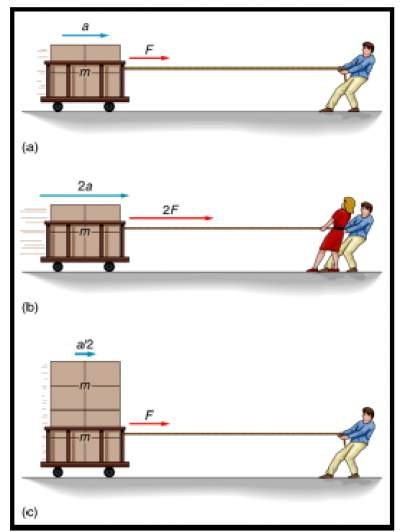
\includegraphics[width=.6 \linewidth]{newton-second.jpg}
    \caption{La deuxième loi de Newton}
    \label{newton_second}
\end{figure}

\newpage

\section{Exercices}
\begin{exercise}
    Une force de \(500[N]\) s'exerce sur une masse de \(40[kg]\). Que vaut l'accélération de cette masse ?
\end{exercise}
\begin{solution}
    \(a=12,5[m/s^2]\)
\end{solution}


\begin{exercise}
    Avec quelle intensité faut-il tirer sur une masse de \(150[kg]\) pour lui communiquer une accélération de \(4[m/s^2]\) ?
\end{exercise}
\begin{solution}
    \(F=600[N]\)
\end{solution}

\begin{exercise}
    Le moteur d'une voiture de \(300[kg]\) lui permet de passer de 0 à \(100[km/h]\) en \(15[s]\). Quelle est la force exercée par ce moteur ? On néglige les frottements.
\end{exercise}
\begin{solution}
    \(F=555,56[N]\)
\end{solution}

\begin{exercise}
    La locomotive d'un train de 750 tonnes, initialement au repos, peut exercer une force motrice de \(65[KN]\) sur celui-ci. Les frottements qui s'exercent sur le train valent \(25[KN]\).
    \begin{enumerate}[a)]
        \item Quelle est la vitesse du train après 180[s] d'accélération ?
        \item Quelle doit être la force à exercer pour maintenir le train en MRU?
    \end{enumerate}
\end{exercise}
\begin{solution}
    \(v_{180}=9,6[m/s]\)
    \(F=25000[N]\)
\end{solution}

\begin{exercise}
    Un cycliste démarre en exerçant une force motrice de \(200[N]\). Après 5[s] d'accélération, la force motrice est réduite à \(40[N]\) pour maintenir une vitesse constante. La masse du cycliste et du vélo est de \(80[kg]\) et on suppose les frottements constants.
    \begin{enumerate}[a)]
        \item Que vaut l'intensité des forces de frottements qui s'exercent sur le cycliste et son vélo ?
        \item Quelle est l'intensité de la résultante des forces qui s'exercent sur le cycliste durant les 5 premières secondes ?
        \item Que vaut l'accélération durant les 5 premières secondes ?
        \item Quelle est la vitesse après les 5 premières secondes ?
    \end{enumerate}
\end{exercise}

\begin{exercise}
    Une voiture dont la masse est de \(1200[kg]\) roule à la vitesse de \(90[km/h]\) sur une route rectiligne. Elle commence à freiner et s'arrête en \(5[s]\).
    Précise le sens, la direction et l'intensité de la force exercée par les freins.
\end{exercise}
\begin{solution}
    \(F=6000[N]\)
    \(\vec{F}\) est de même direction que \(\vec{v}\), mais de sens opposé.
\end{solution}


\begin{exercise}
    Un cycliste de \(75[kg]\), vélo compris, doit exercer une force de \(30[N]\) pour rouler à la vitesse constante de \(20[km/h]\). En combien de temps s'arrête-t-il lorsqu'il cesse de pédaler ?
\end{exercise}
\begin{solution}hello
    \(\Delta t=13,89[s]\)
\end{solution}
